\section{Үр дүн}
\subsection{Front харагдах байдал}

\begin{figure}
	\centering
	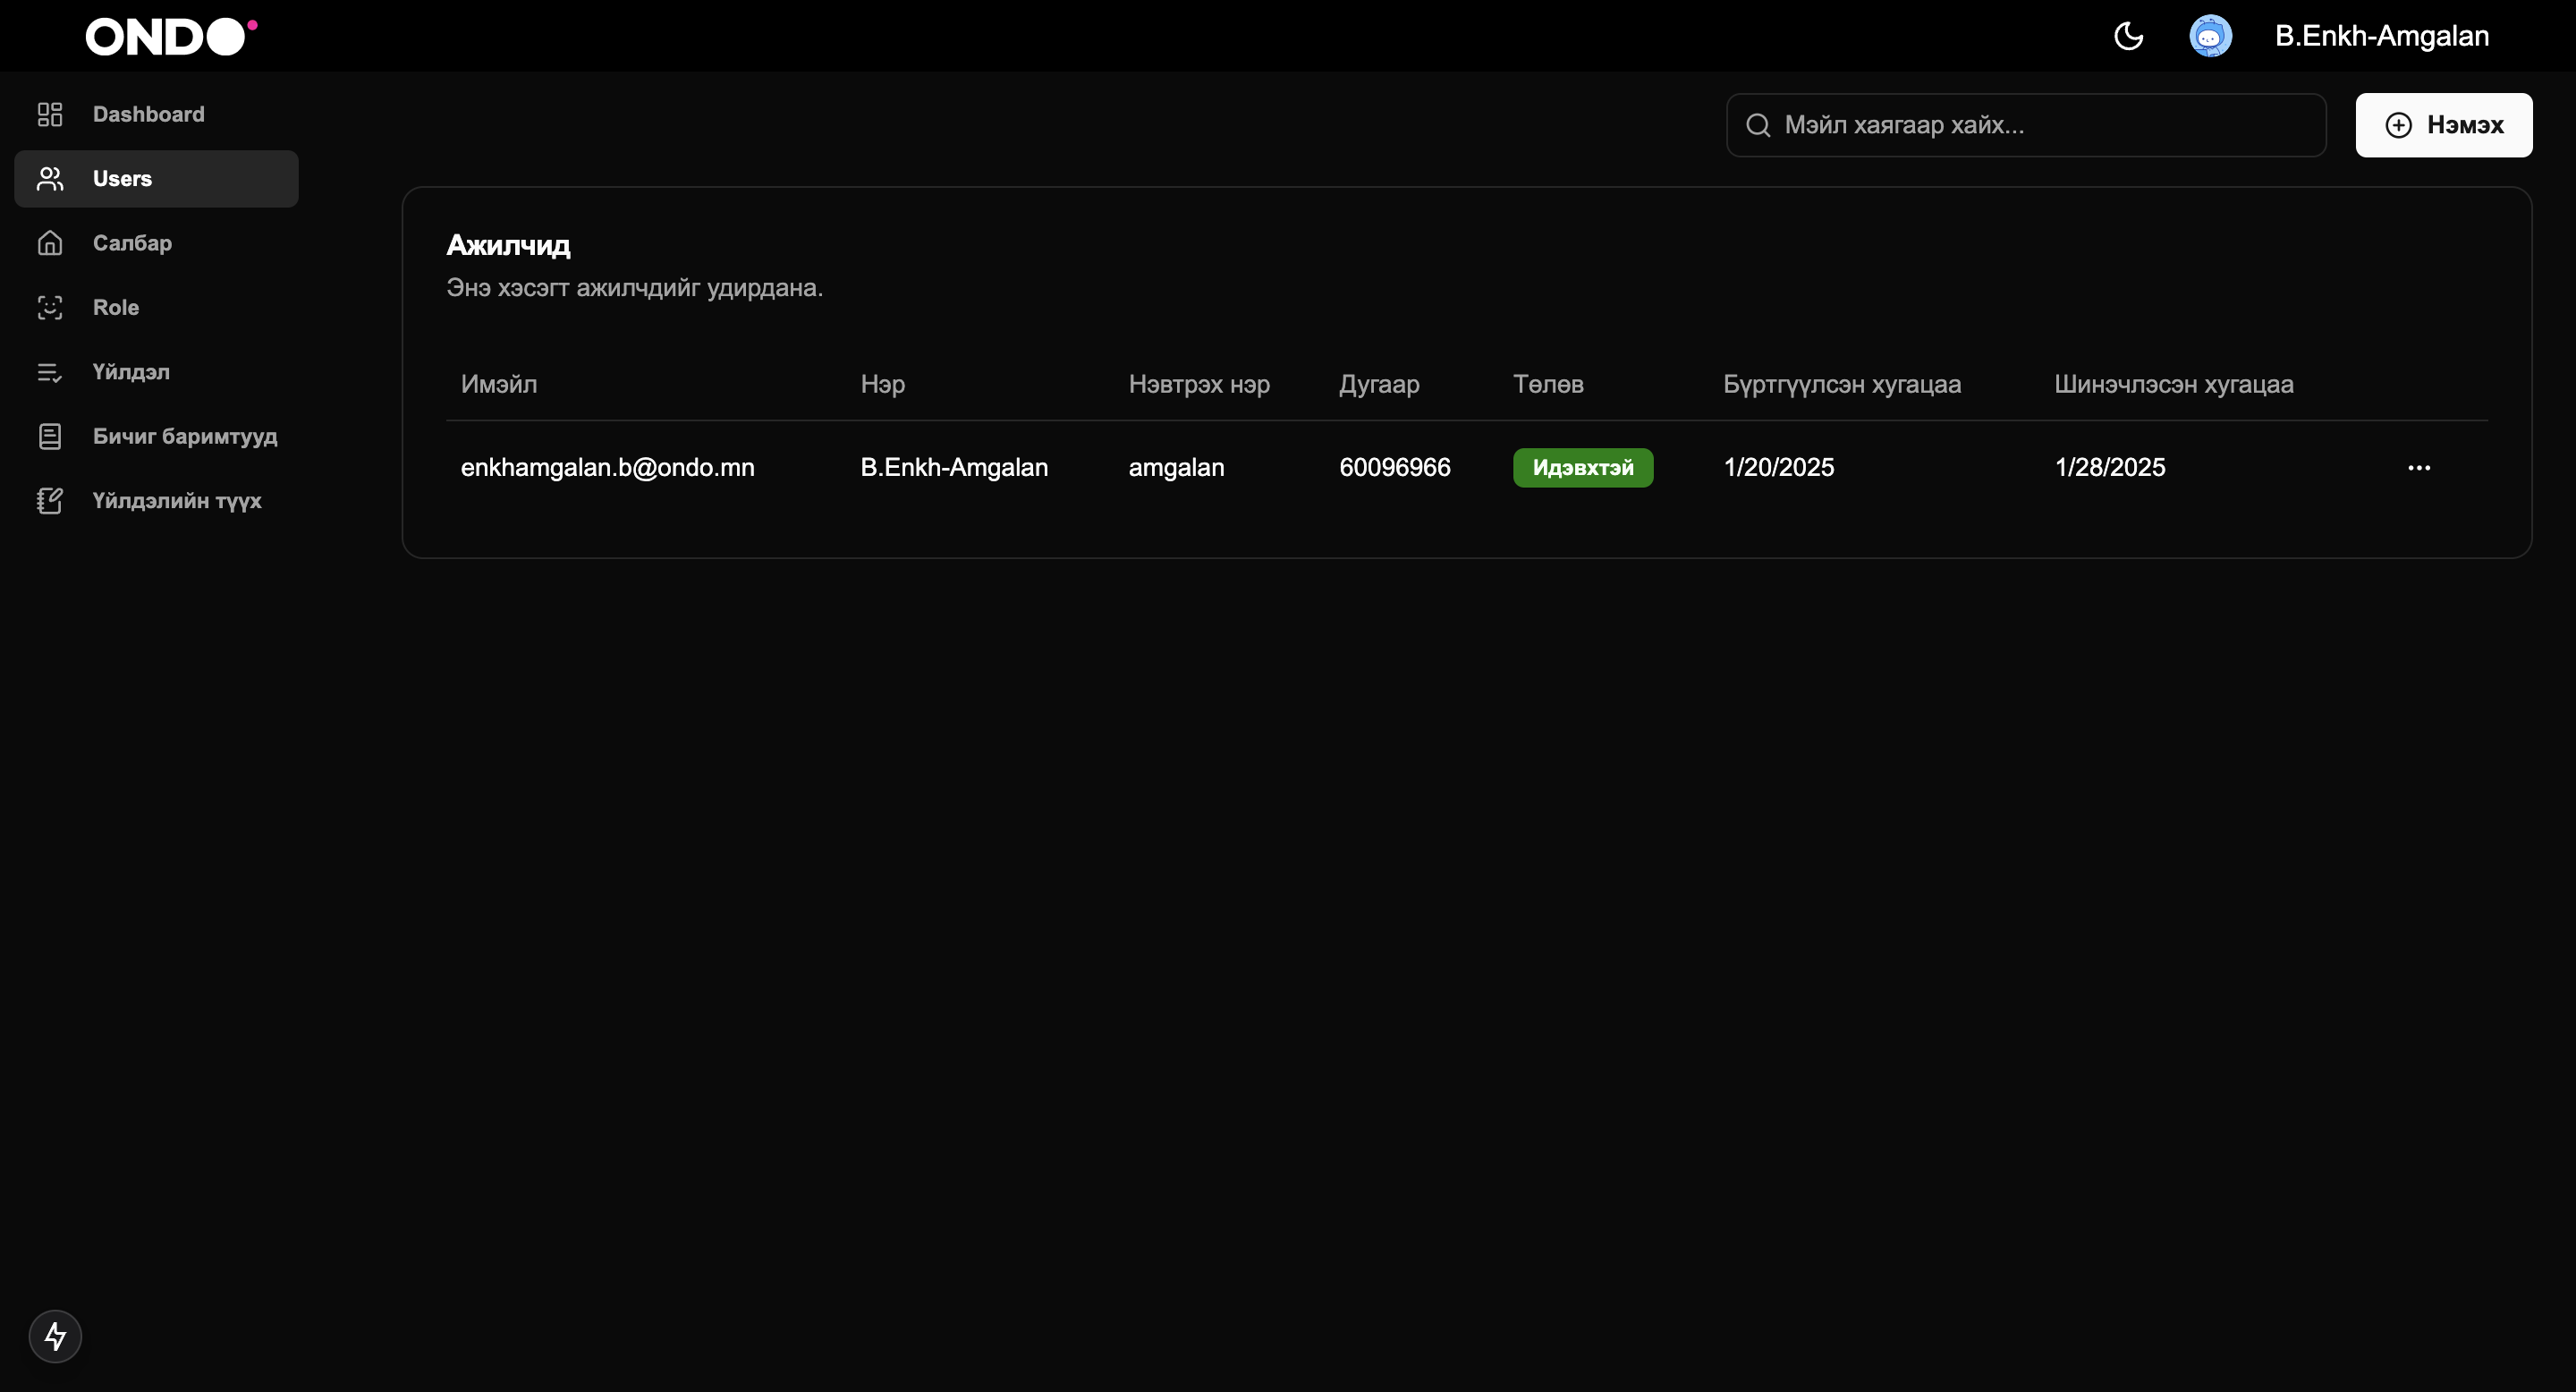
\includegraphics[width=15cm]{images/main.png}
	\caption{Хэрэглэгчидын жагсаалт}
\end{figure}

\begin{figure}
	\centering
	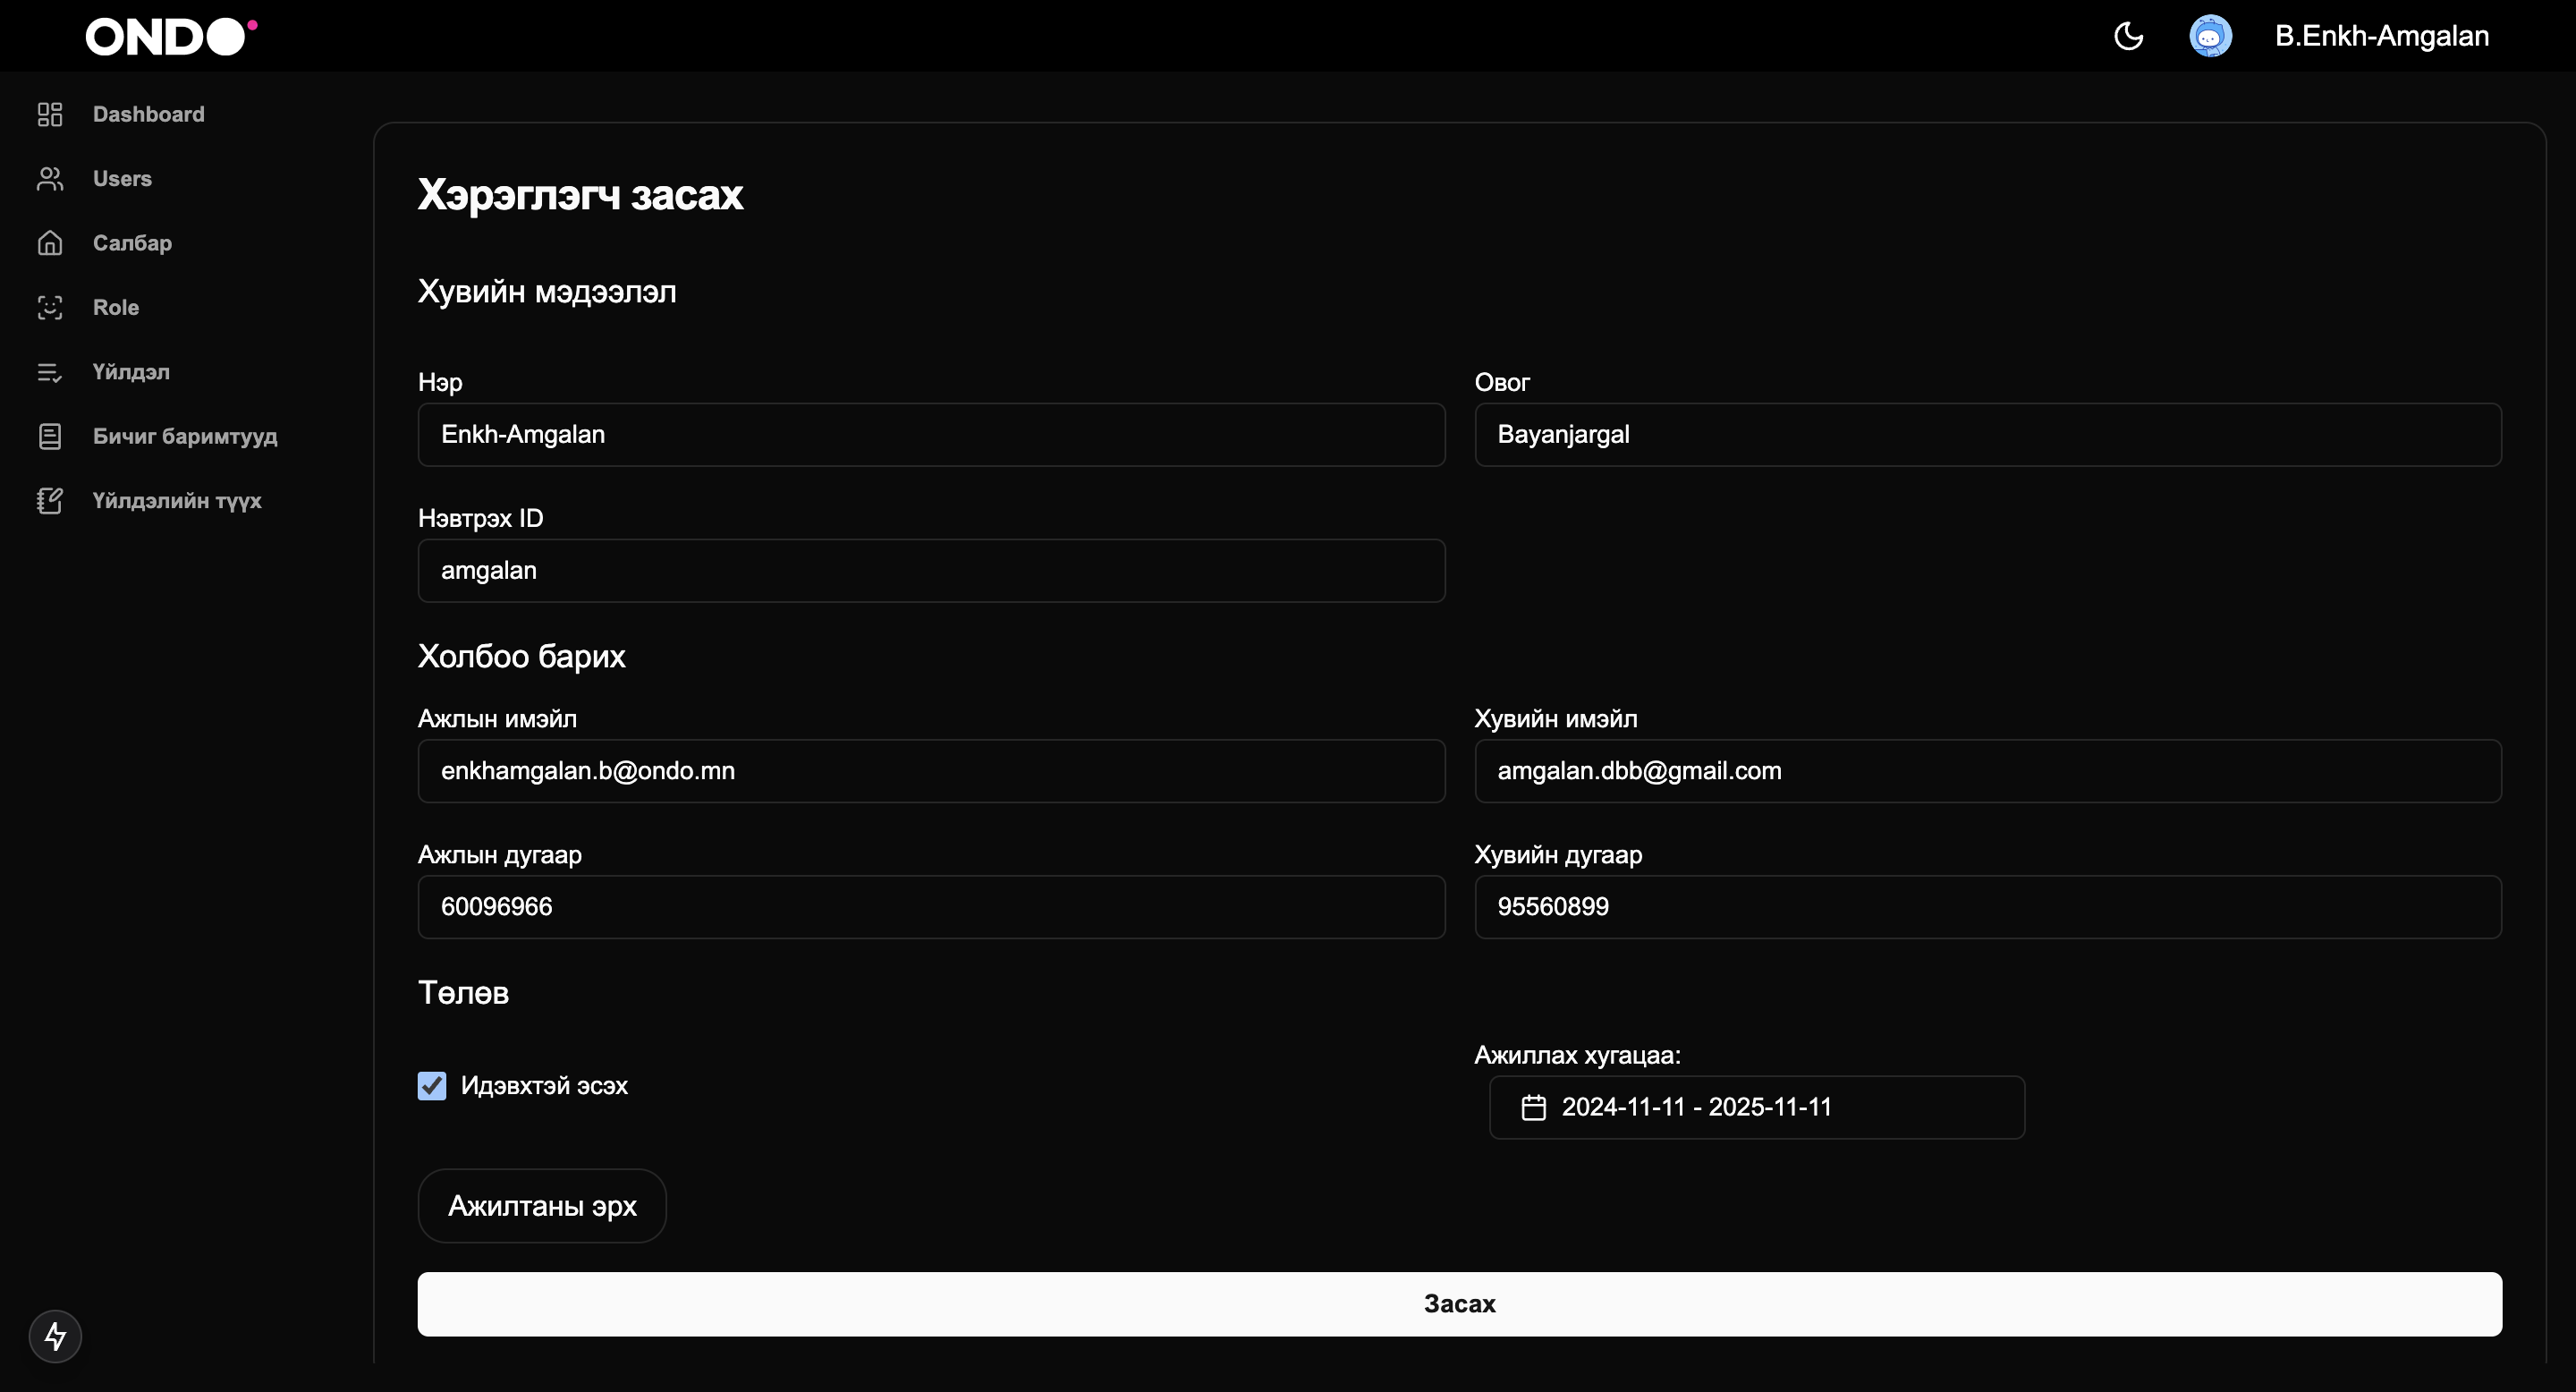
\includegraphics[width=15cm]{images/front.png}
	\caption{Хэрэглэгч засах}
\end{figure}

\begin{figure}
	\centering
	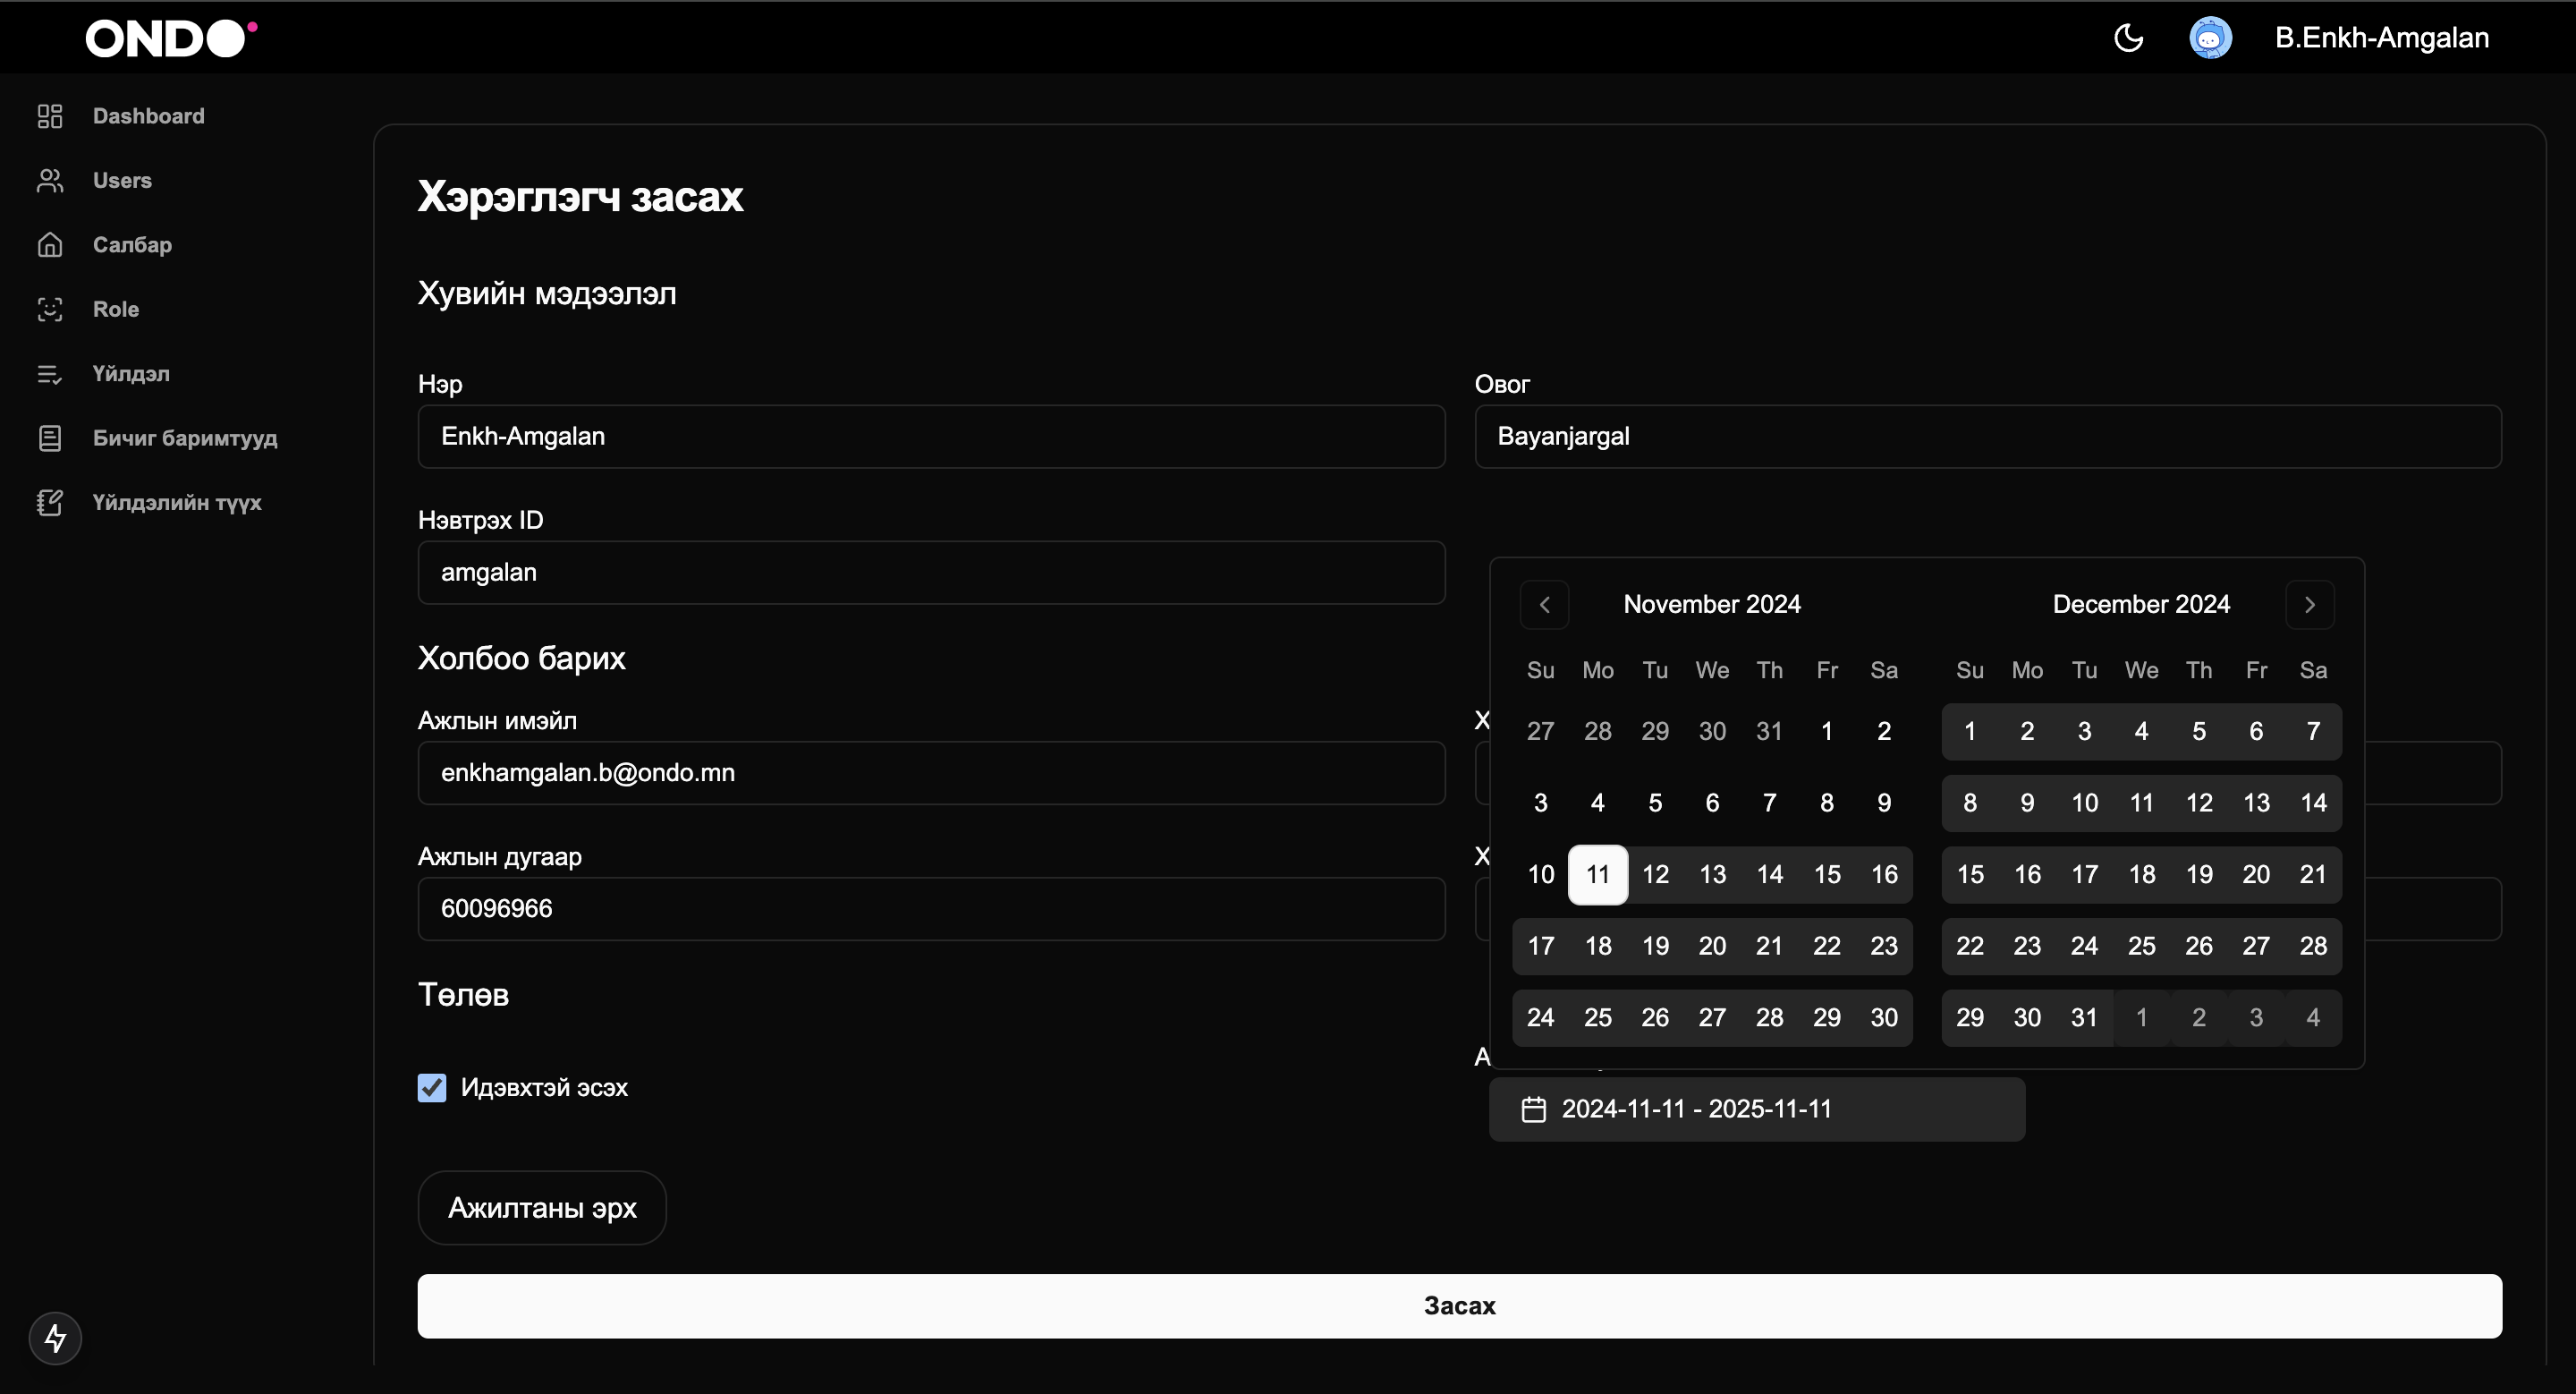
\includegraphics[width=15cm]{images/calendar.png}
	\caption{Өдөр сонгох календар}
\end{figure}

\begin{figure}
	\centering
	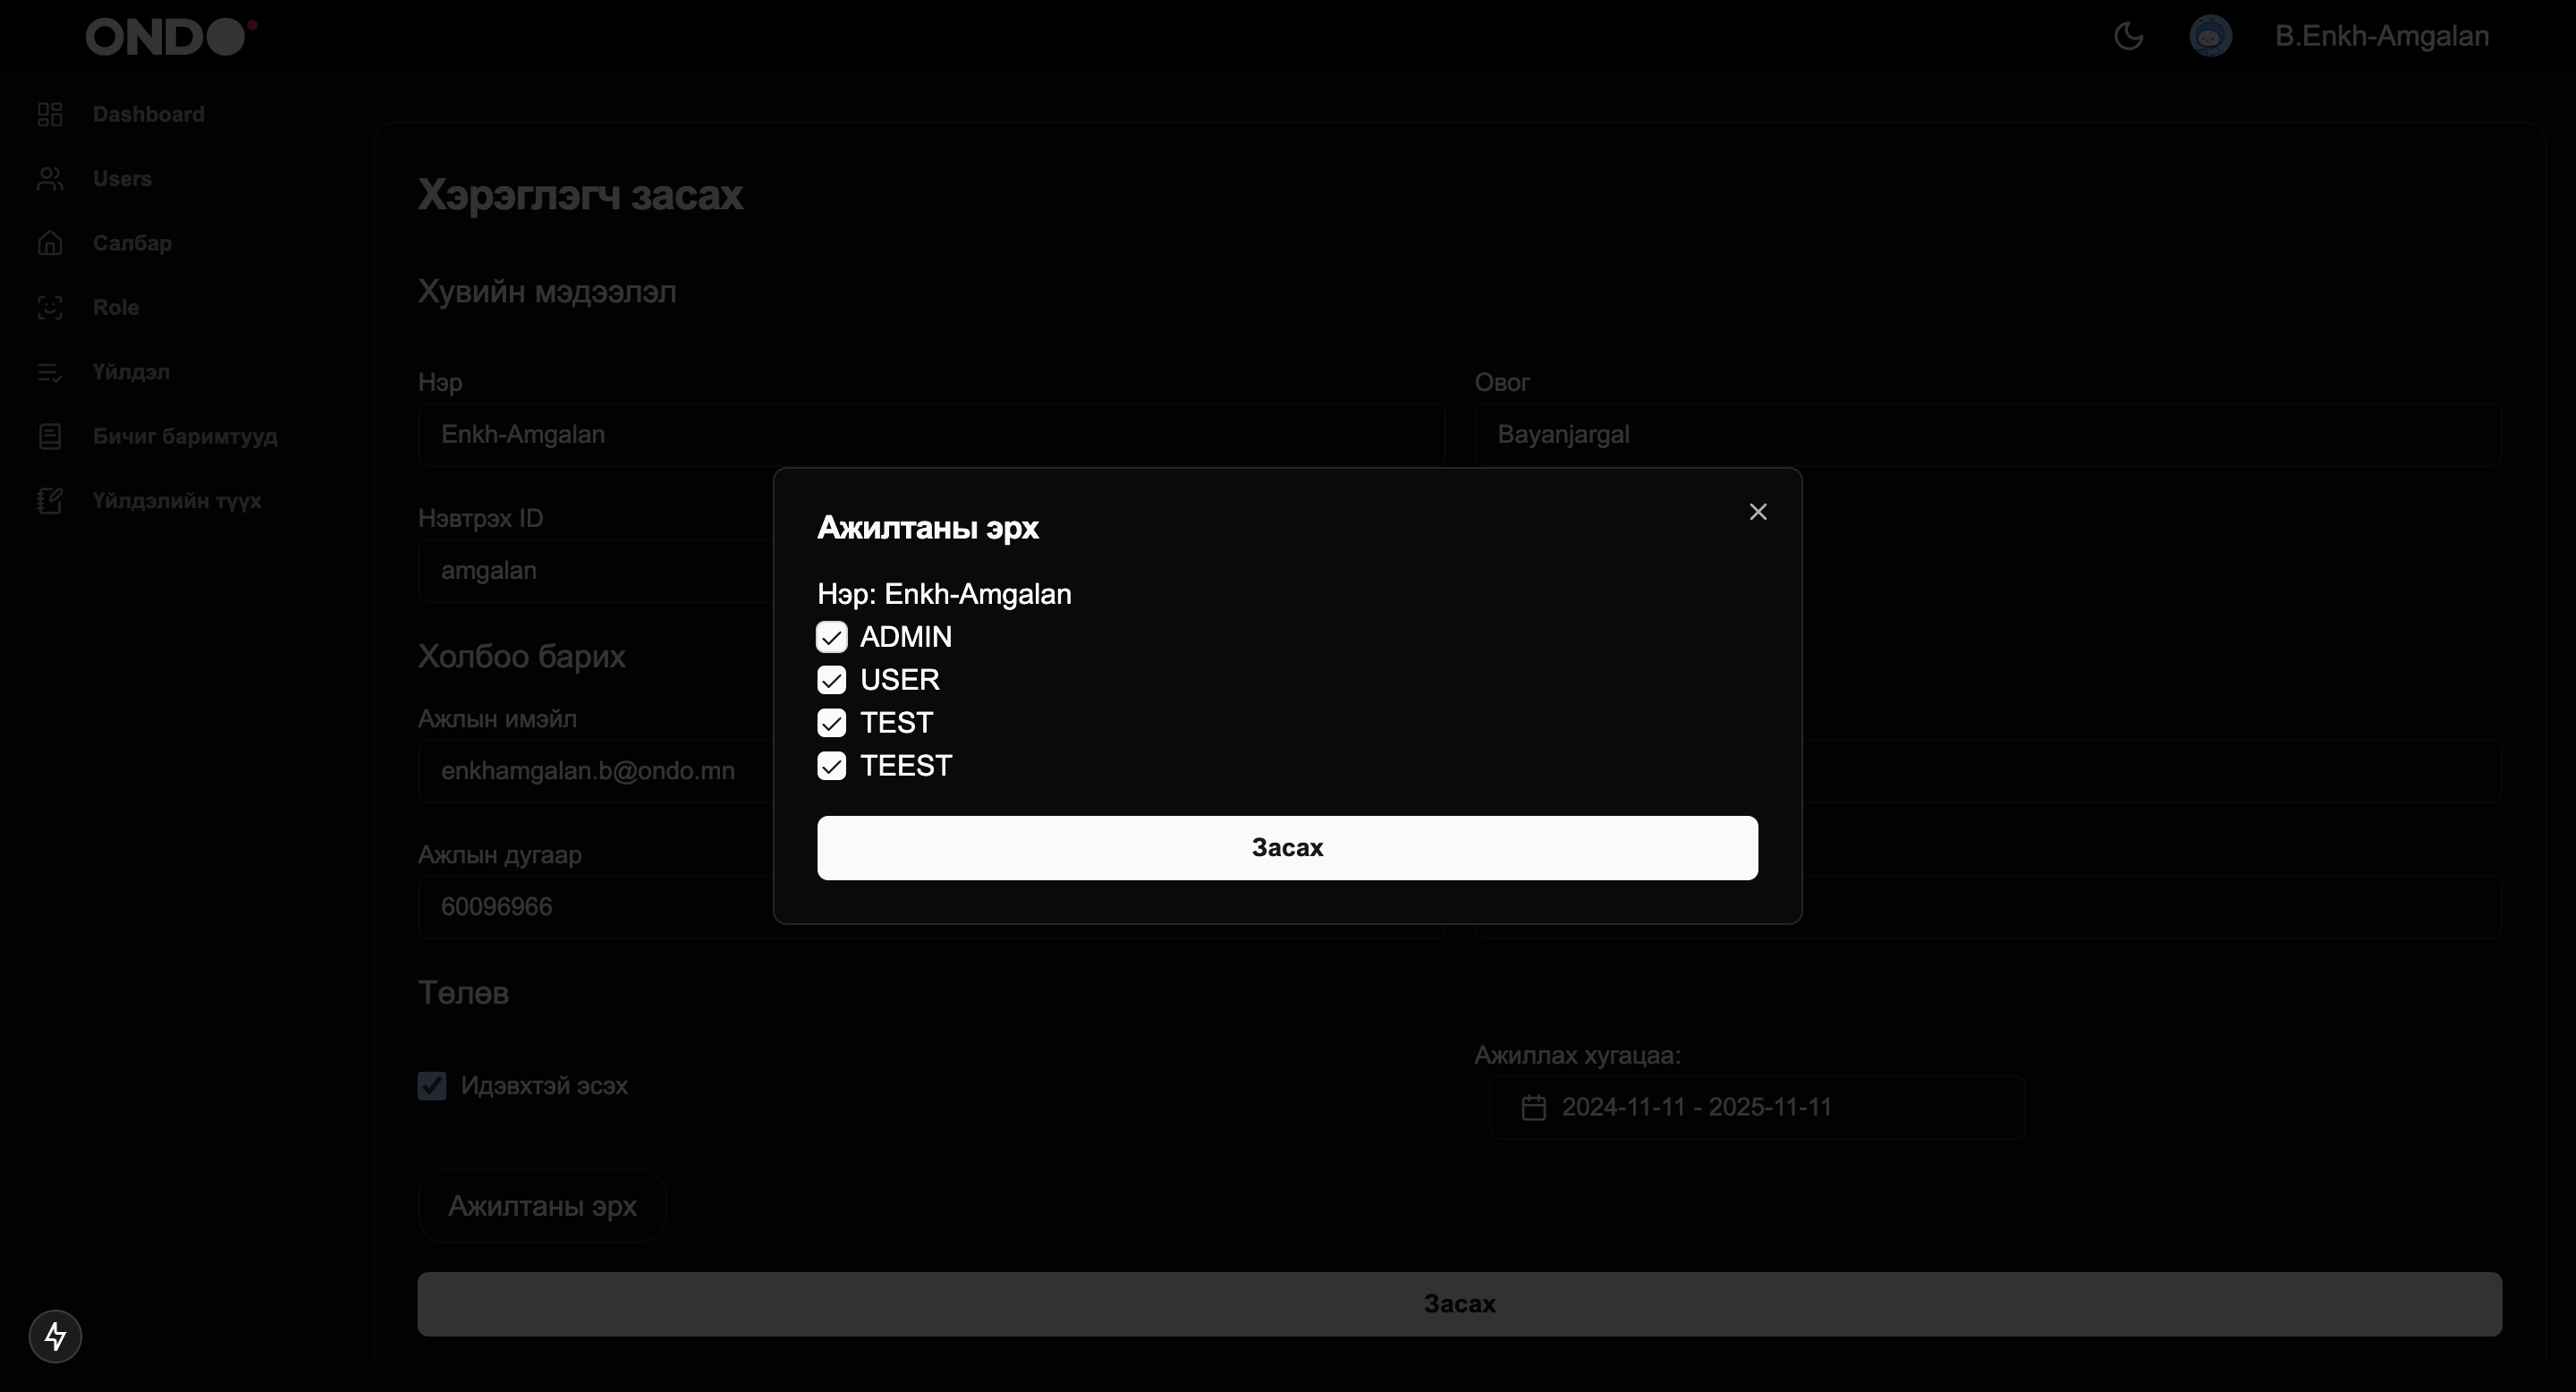
\includegraphics[width=15cm]{images/role.png}
	\caption{Ажилтны эрх сонгох хэсэг}
\end{figure}
\pagebreak

\clearpage

\section{Дүгнэлт}
Миний бие ОНДО ХХК-д 21 хоногийн хугацаатай мэргэжлийн дадлагыг амжилттай гүйцэтгэж дуусгалаа. Уг хугацаанд хичээлийн хүрээнд үзсэн онолын ойлголтуудыг практик дээр туршиж, хэрэгжүүлсэн ба хөгжүүлэлт голчилсон технологийн компанийн ерөнхий үйл ажиллагаа, баг хооронд зохицон ажиллах чадвар, хөгжүүлэлтийн шинэ арга барилуудыг амжилттай эзэмшсэн гэж дүгнэж байна.

\quad Continuous Integration/Continuous Deployment, GITLAB дээрх Feature Branch, Next.js болон Golang түүний сан GIN болон өгөгдлийн сантай ажиллах GORM зэрэг сантай ажиллаж түүний давуу талыг судлан уг хэлээрээ сэтгэж бичих, том асуудлыг олон болгон хувааж багаар, алхам дэс дараатай асуудлыг шийдвэрлэх мөн ашиглаж буй сан, технологийнхоо гарын авлага буюу documentation-тай илүү сайн танилцаж уг технологийнхоо цаана нь буй концептийг хялбараар ойлгох гэх мэт чадваруудыг эзэмшсэн. Үүнийгээ цаашид илүү хөгжүүлж мэргэшсэн Full-Stack хөгжүүлэгч болохоор зорьж байна. 

\quad Дадлагын хүрээнд бүрэн хэмжээний хөгжүүлэлтийн талаар практик ойлголтыг олж авч богино хугацаанд өөрийн хэмжээнд багагүй туршлага хуримтлуулсан.Мөн хийсэн төсөл дээрээ тулгуурлан өөрийн
тайланг бичих туршлагатай болсон. Цаашид сурсан зүйлсээ илүү бататган ирээдүйдээ ашиглахаарзорьж байна. Мэдлэгийн хүрээг минь тэлэхэд үнэтэй хувь нэмэр оруулсан МТЭС-МКУТ-даа болон ОНДО ХХК-д талархал илэрхийлье.